%Latex2e file
\documentclass[12pt,letterpaper]{article}
%\renewcommand{\arraystretch}{2}
%\input{\scrload.tex}
\setlength{\textwidth}{6.5in}
\setlength{\textheight}{9.5in}

\setlength{\oddsidemargin}{-.25in}
\setlength{\evensidemargin}{-.25in}
\setlength{\topmargin}{-.25in}
\pagestyle{empty}

\usepackage{amsmath}
\usepackage{amssymb}
\usepackage{graphicx}

\newcommand{\R}{\ensuremath{{\mathbb{R}}}}
\newcommand{\Z}{\ensuremath{{\mathbb{Z}}}}
\newcommand{\Q}{\ensuremath{{\mathbb{Q}}}}
\newcommand{\N}{\ensuremath{{\mathbb{N}}}}
\newcommand{\C}{\ensuremath{{\mathbb{C}}}}
\newcommand{\Proof}{\noindent {\bf Proof: }}
\newcommand{\QED}{\begin{flushright}QED\end{flushright}}
\newcommand{\Refl}{{\bf Reflexive: }}
\newcommand{\Symm}{{\bf Symmetric: }}
\newcommand{\Tran}{{\bf Transitive: }}
\newcommand{\ep}{\varepsilon}
\newcommand{\ri}{\right|}
\newcommand{\lef}{\left|}
\newcommand{\toR}{\to \R}
\newcommand{\fancy}[1]{#1_{\text{fancy}}}
\newcommand{\pro}[1]{\noindent {\bf #1}}
\newcommand{\prob}[1]{\newpage\noindent {\bf #1}}
\newcommand{\bacon}{\approx}

   
\begin{document}
\begin{flushright}
Nick Kerner

Homework 2

Chapter 2: 9,10,11,13; Major exercise 1
\end{flushright}
\begin{center}
\large{Geometry}\\
\end{center}

\pro{9} In each of the following interpretations of the undefined terms, which of the axioms of incidence geometry are satisfied and which are not?  Tell whether each interpretation has the elliptic, Euclidean, or hyperbolic parallel property. \\

a. "Points" are lines in Euclidean three-dimensional space, "lines" are planes in Euclidean three-space, "incidence" is the usual relation of a line lying in a plane.\\

Incidence axiom 1: This is not satisfied.  In high school geometry, we had skew lines.  Considering two skew lines, we cannot create a Euclidean three-space plane which contains both lines.\\ 


Incidence axiom 2: A Euclidean three-space plane does contain (is incident with) at least two unique Euclidean three-space lines.  This is satisfied.\\


Incidence axiom 3: Here we must have three lines that do not lie in the same plane.  Consider 2 lines in a plane (I2), and pick some other line, parallel to one of these lines, but not in the plane.  This line is clearly not in the same plane.  We have three non-collinear ``points'', I3 is satisfied.\\


Parallel property:

Euclidean parallel property: Given a plane and a line which does not lie on that plane (so, theoretically, they can intersect) the Euclidean parallel property is true if we can find a plane containing our line that is parallel to the given plane.  However, if the line intersects the given plane but does not lie on it, then all planes containing that line do have a line in the given plane and therefore are not parallel to the given plane.  Therefore the Euclidean parallel property is not satisfied here.\\

Elliptical parallel property:  Since we can create two planes which do not intersect (such as the planes created by extending the top and bottom of a Euclidean 3-space cube), we know that the elliptical parallel property is not satisfied here.\\

Hyperbolic parallel property:  Given a plane $l$, let $P$  be a line which does not line on $l$, but intersects it.  As in the Euclidean parallel property section above, there are an infinite number of planes which $P$ lies on, none of which are parallel to $l$.  Therefore the Hyperbolic parallel property is not satisfied. 


Given a plane, we can find a plane parallel to it, but we cannot find a plane parallel to it that is incident with just any old line.  None of these properties are satisfied.

\newpage

b. Same as in part (a), except that we restrict ourselves to lines and planes that pass through a fixed point O.

Incidence axiom 1: As all lines pass through O, any two lines will form a unique Euclidean 3-space plane, so this axiom is satisfied.\\


Incidence axiom 2: Given a plane containing O, we can create perpendicular lines through O in that plane, therefore the second axiom is satisfied.\\


Incidence axiom 3: Consider a Cartesian coordinate system with O as the origin.  The axes consist of three lines which cannot be used to create a single plane.  Therefore the third axiom is not satisfied.\\


Parallel property:

Euclidean parallel property: As with part a, given a plane l and a line P that does not lie on l, we know that P intersects l at O.  Additionally, we know that the intersection of two three-space planes forms a line.  Therefore this parallel property is not met.\\

Elliptical parallel property: Since the intersection of two three-space planes forms a line and since all of our planes intersect at O, the intersection of any two planes will be a line, so there are not parallel "lines". Therefore this axiom is satisfied.\\

Hyperbolic parallel property: Since there are no parallel "lines", there are obviously not two or more parallel "lines" given a plane and a line which does not lie on it. \\




\newpage 

c. Fix a circle in the Euclidean plane.  Interpret "point" to mean a Euclidean point inside the circle, interpret "line" to mean a chord of the circle, and let "incidence" mean that the point lies on the chord.  (A chord of a circle is a segment whose endpoints lie on the circle.)\\


Incidence axiom 1: Given a point P and a point Q both inside the circle, we can construct a unique Euclidean line incident with both of them in the Euclidean plane. Since both of these points are inside the Euclidean circle, we know that the Euclidean line contains a segment which is a chord.   Consider the idea that this segment is not unique.  Then there must be another Euclidean line through P and Q which violates I1.  Therefore there is a unique chord containing these two points.  \\


Incidence axiom 2: Given a chord, consider the line containing that chord.  The line intersects the circle at two points, call them $A$ and $B$.  The segment connecting these two points can be bisected, call this point $C$, and the segment $AC$ can be bisected, call this new point $D$.  Note that $C$ and $D$ are inside the Euclidean circle and are therefore ``points'' on our chord $AB$.  Therefore the axiom is satisfied. \\


Incidence axiom 3: Consider a cartesian coordinate system with the center of the circle as the origin.  The axes are perpendicular to each other in the Euclidean plane. Consider the chords $AO$ and $BO$ connecting the center and the circle (along different axes). Then we can bisect $AO$ finding point $X$ and bisect $BO$ finding point $Y$.  Note that we cannot connect $X,Y$ and $O$ in the Euclidean plane with a line.  Therefore we cannot create a chord containing these three points, so they are non-collinear in our new model and therefore the axiom is satisfied. \\

Parallel property: Given a chord l and a point P in the circle not on l, note that in the Euclidean plane we can create multiple lines that go through P, and which intersect the line extended from l, but do not intersect it inside the circle.  Therefore the chords from each of these lines do not intersect l, but do go through P. Therefore there are multiple parallel chords or ``lines'' through P.\\

Euclidean parallel property: The parallel ``line'' is not unique, this is not satisfied.\\

Elliptical parallel property: Parallel ``lines'' can be found, this is not satisfied.\\

Hyperbolic parallel property: Consider the chord l and point P.  Let l be the segment $AB$ in the Euclidean plane.  Then consider the line through $BP$. This intersects the circle at some other point $D$ which is not $A$.  Any point on the arc of the circle from $A$ to $D$ can be used with $P$ to create another chord which does not intersect $AB$.  Since there are an infinite number of points on the arc between $A$ and $D$, there are an infinite number of lines parallel to l. \\




\newpage

d. Fix a sphere in Euclidean three-space.  Two points on the sphere are called antipodal if they lie on a diameter of the sphere;  e.g., the north and south poles are antipodal.  Interpret a "point" to be a set $\{P,P'\}$ consisting of two points on the sphere that are antipodal.  Interpret a "line" to be a great circle on the sphere.  Interpret a "point" $\{P,P;\}$ to "lie on" a "line" C if both P and P' lie on C (actually, if one lies on C, then so does the other, by the definition of "great circle".)\\

Incidence axiom 1: Given two unique ``points'' we can create a great circle containing all four of their Euclidean points.  Additionally, we can only create a single, unique great circle that does this.  Therefore there is a ``unique'' line that connects these two ``points''.\\

Incidence axiom 2: Given a great circle we can create a pair of perpendicular lines that intersect at the center of the circle in the same Euclidean plane as the circle. These lines intersect the circle and create chords in the circle, call them $AB$ and $CD$.  The two ``points'' $\{A,B\}$ and $\{C,D\}$ are on the same ``line''.  Since we were able to find said ``points'', the axiom holds in this model.\\


Incidence axiom 3:Consider a three dimensional cartesian coordinate system through the center of the sphere.  The three ``points'' found where the axis intersect the sphere cannot have a single great circle contain them all. Therefore this axiom is satisfied.\\


Parallel property: Given any two great circles or ``lines'', we know that they intersect.  Since the intersect is a point and its antipodal point we know that they intersect at a ``point''.  Therefore there are no parallel ``lines''.\\

Euclidean parallel property: Not satisfied\\

Elliptical parallel property: Satisfied\\

Hyperbolic parallel property: Not satisfied\\







\prob{10} 

a. Show that when each of two models of incidence geometry has exactly three "points" in it, the models are isomorphic.\\

\Proof

Consider two models each with 3 points.  Let the first model have the points A,B,C and let the second model have the points X,Y,Z.  \\

\noindent Notice I can make this 1-1 correspondence between points:

\noindent A$\leftrightarrow$X\\
B$\leftrightarrow$Y\\
C$\leftrightarrow$Z\\

But we must identify the lines of each model. By I1, each pair of points must have a line.  So AB, BC and AC are lines, but are they distinct?  

By I3 we know that they are distinct lines. \\ 

However, can there be more lines?  By I2 all lines must have 2 points, but we have exhausted every possible pair! Therefore there can be no more lines. \\

Therefore AB, BC and AC are our only lines.  Similarly, XY, YZ, and XZ are the only lines for the other model.  Notice we can make this 1-1 correspondence between lines of the different models.\\

\noindent AB$\leftrightarrow$XY\\
BC$\leftrightarrow$YZ\\
AC$\leftrightarrow$XZ\\

$\Rightarrow$
Now we must show that since A is incident with AB and AC, that X is incident with XY and XZ; that since B is incident with AB and BC, that Y is incident with XY and YZ; and finally that since C is incident with BC and AC that Z is incident with YZ and XZ.  Based on our naming scheme for lines, this is obviously the case. \\


$\Leftarrow$
This is essentially the same as above.\\


 Therefore these models are isomorphic.
\QED

\newpage 



b. Must two models having exactly four "points" be isomorphic?  If you think so, show this;  if you think not, give a counterexample.\\

\noindent {\bf Counterexample:}

Consider these two models. The first has points A,B,C and D, the other has points T,X,Y and Z.  We must show that both are models of incidence geometry.\\

\noindent First model:

Let the first contain lines ABC, AD, BD and CD.  Note every pair of points has a unique line so I1 is satisfied, every line has at least 2 points so I2 is satisfied, and A, B, and D are not collinear so I3 is satisfied. Therefore this is a model of incidence geometry.\\

\noindent Second model: 

Let the second model contain lines TX, TY, TZ, XY, XZ and YZ.  Note every pair of points has a unique lines so I1 is satisfied, every line has at least 2 points so I2 is satisfied, and T, X, and Y are not collinear so I3 is satisfied. Therefore this is a model.\\


Assume to the contrary that we have some 1-1 correspondence between the points, and another between the lines such that if a point is incident with a line in one model, the point it maps to is incident with the point the line maps to (definition of isomorphism).  

So we know that A, B and C each map to a point in $\{T,X,Y,Z\}$. Then suppose that ABC maps to l in the second model.  Since $A\in ABC$, $B\in ABC$, and $C\in ABC$ then all three corresponding points in $\{T,X,Y,Z\}$ must be incident with l.  However, every line in the second model has two points.  Without loss of generality, suppose A and B map to points incident with l, call them A' and B'.  Since our mapping is a bijection (by assumption), C cannot map to A' or B'.  Therefore C must map to a point not on l.  Contradiction.  Therefore these two models are not isomorphic.





\newpage 

c. Show that the models in Exercises 9(b) and 9(d) are isomorphic.  (Hint:  Take the point O of Exercise 9(b) to be the center of the sphere in Exercise 9(d) and cut the sphere with lines and planes through point O to get the isomorphism.)\\


\Proof

Take the point O of Exercise 9(b) to be the center of the sphere in Exercise 9(d)

Given a line, P, in the first model, let the points intersecting the sphere be the ``point'' in 9(d) that P maps to.  We know this is possible since a line going through the center of a sphere will contain a diameter of that sphere and then ends of the diameter segment will be antipodal.  

Similarly, given a plane, l, in the first model, let the great circle which lies in that plane be the ``line'' that l maps to.  

We must show that this relations are 1-1 and that if a line in the first model is in a plane in the first model, then the antipodal pair or ``point'' of the second model is in the great circle or ``line'' that the plane maps to.\\

\noindent Case 1: bijection of points

Injective: Given two lines x and y each through O such that both map to the same ``point'', we know that both of these lines intersect the sphere in the same two places.  By the first axiom of incidence geometry, they are the same line.  Therefore $x = y$.

Surjective: Given a ``point'' in the second model that corresponds to a pair of points in Euclidean three space.  Also we know that these points are antipodal on a sphere.  Therefore we can connect them and the line will go through O and therefore is a line in the first model.  The line in the first model maps to the original given ``point'' based on the way the mapping was defined.\\


\noindent Case 2: bijection of lines

Injective:  Given two planes through O that map to the same great circle we know that each circle in 3 space is incident with only 1 plane.  Therefore since both planes map to the same great circle, they are the same plane.  Therefore this mapping is injective.

Surjective:  Given a great circle of the sphere, we know that it is a circle in 3 space and that circles always lie in some plane.  Also, we know that the center of the circle is the center of the sphere, that is, O, so the plane the circle lies in goes through O.  Therefore the plane the circle lies in is a ``line'' in the first model, and by our mapping defintion maps to our circle.\\

\newpage 

$\Rightarrow$
Given a plane in the first model (through point O) and a line that lies in that plane (through point O), we know that the plane maps to a great circle of the sphere.  This circle (by definition) can be drawn in the plane.  The line that lies in the plane goes through O and therefore intersects the circle lying in the plane.  Additionally, it is clear that the line intersects the circle in the same place that it intersects the sphere.  These two places are a pair of antipodal points which compose the ``point'' in the second model which the Euclidean line mapped to.  Therefore it has been show that since the line was incident with the plane, the ``point'' the line mapped to was incident with the ``line'' the plane mapped to.

$\Leftarrow$
Given a pair of antipodal points and a great circle incident with this ``point'' (second model), we know that this circle maps to the plane it lies in.  Additionally, we know this pair of points are on the circle.  Therefore we know that the line connecting these two points is incident with the circle lying in the plane, and therefore it lies in the plane.


\QED





\prob{11} Invent a model of incidence geometry that has neither the elliptic, hyperbolic, nor Euclidean parallel properties. These properties refer to any line l and any point P not on l.  Invent a model that has different parallelism properties for different choices of l and P.  (Hint:  Five points suffice for a finite example, or you could find a suitable piece of the Euclidean plan for an infinite example, or you could refer to a previous exercise.  Or invent a fourth example.)\\



Consider a model with 5 points, $A,B,C,D$ and $E$ where $A,B$ and $C$ are all on the same line and every other line consists of 2 points.  So $AB = AC = BC$, $AD$, $AE$, $BD$, $BE$, $CD$ and $CE$ are all of the lines (where each line listed is distinct from the others). First we must show this is a model.  \\

\noindent I1: Given any 2 points, we can find a line which contains those two points by merely searching the list of lines above. 

\noindent I2: Note that all lines have been listed.  The way in which they have been listed clearly shows they all have 2 points.

\noindent I3: Note that $A, B, C$ and $D$ are not on the same line as the only line that contains both $B$ and $D$ is $BD$ and this line does not contain $A$.

Therefore this is a model of incidence geometry.  Now we must show that it does not exhibit the hyperbolic, Euclidean, or elliptic parallel properties.\\




\noindent Elliptic, Hyperbolic:\\

Consider the line $ABC$.  For a line to be parallel to this line it must be a distinct line and it must have points not incident with the line. Therefore it cannot contain points $A,B$, or $C$.  Therefore it can only contain points $D$ and $E$.  Therefore, since by the second axiom all lines must have two points, the only line that is parallel to $ABC$ is $DE$.  This appears to exhibit the Euclidean parallel property in this one case, so this model does not exhibit the Elliptical or hyperbolic parallel properties.  \\

\noindent Euclidean: \\

Now consider the line $AD$. Note that neither $BE$ or $CE$ have points in common with $AD$ and that $AD \neq BE \neq CE$.  Therefore both of these lines are parallel to $AD$ so we exhibit the hyperbolic parallel property.  Therefore this model does not exhibit the Euclidean parallel property.  






\prob{13} Suppose that in a given model for incidence geometry, every "line" has at least three distinct "points" lying on it.  What is the least number of "points" and the least number of "lines" such a model can have?  Suppose further that the model has the Euclidean parallel property, i.e., is an affine plane.  Show that 9 is now the least number of "points" and 12 the least number of "lines" such a model can have.\\
 
 
\noindent A,B,C; AB,AC,BC:\\

There exists 3 non-collinear points (I3), so we have 3 points, A,B, and C.  Each pair of points makes a line (I1), so we have lines AB, AC, and BC.  \\

\noindent D; ABD:\\

Each line must have 3 points (modified I2), so to satisfy this property we must introduce new points as A, B, and C are not collinear (I3). So we need a new point to extend AB, call it D.  So we have line ABD.  \\

\noindent E; ACE:\\

Also we must extend AC (modified I2).  By I1, if A or C are already on a line with another point, it cannot be on another line with that point.  Because of A, we cannot use points B or D as A lies on ABD.  Therefore we need a new point, call it E.  So we have a line ACE.\\


\noindent F; BCF:\\

Similarly, we must extend BC (modified I2).  By I1, if B or C are already on a line with another point, it cannot be on another line with that point.  Because of B, we cannot use points A or D (line ABD).  Because of C we cannot use E (line ACF).  Therefore we need a new point, call it F. \\

\noindent G; BEG:\\
 
By I1 we know that B and E are incident with a unique line.  By our modified I2 we must have a third point on this line.  By I1, if B is already on a line with another point, it cannot be on another line with that point.  Therefore we cannot use A,C,D, or F in the construction of this new line (B is on ABD and BCF).  However, we have run out of points.  So we need a new point, call it G. So BEG is another line. \\
 
I would like to imagine at this time that we have enough points for this model.  Till this point we have been forced to add points to our model repeatedly in an attempt to satisfy our axioms, however, if we can satisfy the axioms without adding more points, then we have the minimum number of points. \\  
 
\noindent AFG:\\

Now we know that A and F must be incident with a line (I1).  By our modified I2 we must have a third point on this line.  By I1, if A or F is already on a line with another point, it cannot be on another line with that point. Because of A, we cannot use points B,D,C, or F (lines ABD and ACE).  Therefore the only point that will work is point G.  So we have line AFG. \\

\noindent FDE:\\

Now we know that F and D must make a line (I1).  By our modified I2 we must have a third point on this line.  By I1, if D or F is already on a line with another point, it cannot be on another line with that point.  Because of D, we cannot use points A or B (ABD) and because of F we cannot use C or G (BCF and AFG).  Therefore the only point we could use is E.  So we have line FDE.

\noindent DCG:\\

Now we know that C and D must make a line (I1).  By our modified I2 we must have a third point on this line.  By I1, if D or C is already on a line with another point, it cannot be on another line with that point.  Because of D, we cannot use points A,B,E, or F (ABD and FDE).  Therefore the only point we could use is G.  So we have line DCG.\\


Our current lines are ABD, ACE, AGF, BCF, BEG, CDG and FDE.  Now we must confirm that we have a model.\\

I1: Given a pair of points, we can search the list of 6 lines above and find that there is exactly one line containing that pair.  Therefore I1 is satisfied. \\

I2: There are three points on every listed line.\\

I3: A,B, and E are not collinear.\\

We have 7 points and 7 lines and we have satisfied all 3 axioms. 


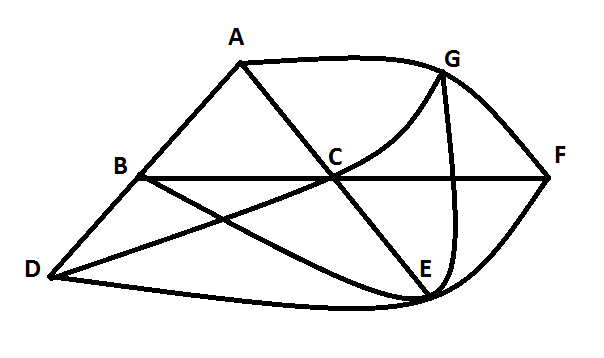
\includegraphics[width=3in]{lines.png}




\newpage 
Part 2:  Suppose we have I1, modified I2, I3 and the Euclidean parallel property. \\

\Proof


By I3 we have 3 non-collinear points, call them A,B and C. By I1, AB is a unique line, by I2 we must have 3 points and by I3 we cannot use point C.  So we need a third point call it D.  So we have ABD. By the Euclidean parallel property we must have a parallel line through C.  Since A,B,C, and D are our only current points and since we cannot use A, B or D (definition of parallel) we must have 2 more points call them E and F.  So we have parallel lines ABD and CEF.  By I1, we have lines AC, AE, and AF.  These must each have a third point (I2) but cannot use points from ABD or CEF as it would imply (I1) that they are the same as ABD or CEF respectively and that would mean that ABD and CEF intersect at A.  As they are parallel they cannot do this (contradiction under Euclidean parallel property).  Similarly, AC, AE, and AF must all use different third points or they would be the same as they would share A and a third point (I1), thus forcing two points from CEF to be the same point, which would be a contradiction.  Therefore call these third points G,H, and I. So we have ACG, AEI, and AFH.  \\



This gives us 9 points.  If we add no more points and come to 12 lines while satisfying all of the axioms, we are done.  If we are attempting to complete a line (we know a pair of 2 points must have a third point but don't know which point is that third point) and there is only 1 point in our set of 9 points that will work we will use that point.  This choice is valid if we satisfy all of the axioms without going out of our set of 9 points. \\


\noindent BEH:\\

B and E must have a line incident with them and it must have 3 points (I1, I2).  We know by I1 that if C or B lie on the same line as one of our other points we cannot use that other point as this would make ABD and CEF out to be the same line.  Therefore we must choose a point from $\{G,H,I\}$ to complete our line.  Suppose we choose I.  Then BEI = AEI by I1, and again ABEI = ABD by I1, so E is incident with ABD, so ABD and CEF are not parallel.  Contradiction, so we cannot choose I.  We are left with two choices then.  Both other choices, G and H are in a line with A (a line that does not go through E or B, and could not or else it would yield a contradiction).  Additionally, both of these other lines (ACH, AFG) go through some other point of CEF.  As such, choosing one will not make a different (our choices have a symmetry to them, and will yield isomorphic models if we continued down both routes).  So without loss of generality, choose H, so we have line BEH.\\    




\noindent DEG:\\

D and E must also have a line incident with them and it must contain 3 points (I1,I2).  By I1 we cannot choose a point that is already on a line with D or E so we cannot choose points from ABD, CEF, AEI, or BEH.  So we must choose G.  Therefore we have line DEG.\\

\noindent GHI:\\

Note that by the Euclidean parallel postulate, we must have a line parallel to CEF through H.  Suppose this is a preexisting line.  The only line parallel to CEF currently (all others intersect it) is ABD.  If $H\in ABD$ then ABD = BEH (I1).  Therefore ABD and CEF are not parallel.  Contradiction.  Therefore there must be some other line parallel to CEF through H (EPP) and it must contain 3 points (GHI).  However, there are only 3 points in our model that are not incident with CEF or ABD. These are GHI, so this will be our line.\\

\noindent DFI:\\

D and F must also have a line incident with them and it must contain 3 points (I1,I2).  By I1 we cannot choose a point that is already on a line with D or F so we cannot choose points from ABD, CEF, AFH, or DEG.  So we must choose I.  Therefore we have line DEI.\\



\noindent DCH:\\

D and C must also have a line incident with them and it must contain 3 points (I1,I2).  By I1 we cannot choose a point that is already on a line with D or C so we cannot choose points from ABD, CEF, ACG, or DFI.  So we must choose H.  Therefore we have line DCH.\\

\noindent BFG:\\

B and F must also have a line incident with them and it must contain 3 points (I1,I2).  By I1 we cannot choose a point that is already on a line with B or F so we cannot choose points from ABD, CEF, BEH, or DFI.  So we must choose G.  Therefore we have line BFG.\\


\noindent BCI:\\

B and C must also have a line incident with them and it must contain 3 points (I1,I2).  By I1 we cannot choose a point that is already on a line with D or C so we cannot choose points from ABD, CEF, ACG, or DCH.  So we must choose I.  Therefore we have line BCI.\\


\newpage 

Now we have piece by piece constructed 12 lines and 9 points, only adding them when we had no other choice but to add them. However, we must still show that this is a model of incidence geometry and that the Euclidean parallel postulate is met.  \\

\noindent I1: Given a pair of points, we can look at the 12 defined lines above and see by inspection that there is a unique line incident with both points in that pair. \\

\noindent I2: All 12 lines mentioned have 3 points on them.\\

\noindent I3: A,B, and C are not on the same line and it would lead to a contradiction if they were.\\

\noindent Euclidean parallel postulate:  Given a line, there are 3 points on that line and 6 points not on that line.  Additionally, those 6 points divide into 2 lines parallel to each other.  These are those sets of lines.\\

\noindent $ABD || CEF || GHI\\
ACG || BEH || DFI\\
AFH || BCI || DCG\\
AEI || BFG || DCH$\\

Note that in stating all the sets of parallels, we are satisfying the Euclidean parallel postulate.  Given a line and a point not on that line, we know that the point is one of the 6 points contained in one of the other two lines, and only in one of the other two lines.  We have exhaustively listed all sets of parallel lines, so there is clearly only one parallel to a given line through a given point not on that line. 

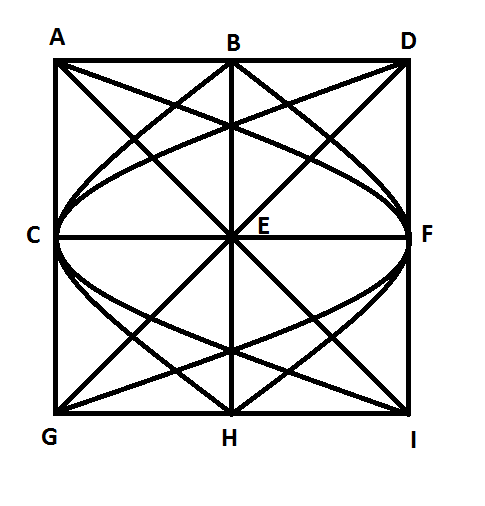
\includegraphics[width=2in]{lines2.png}






 
 
\prob{Major Exercise 1} Consider the following interpretation of incidence geometry.  Begin with a punctured sphere in Euclidean three-space, i.e., a sphere with one point N removed.  Interpret "points" as points on the punctured sphere.  For each circle on the sphere passing through N, interpret the punctured circle obtained by removing N as a "line." Interpret "incidence" in the usual sense of a point lying on a punctured circle.  Is this interpretation a model?  If so, what parallel property does it have?  Is it isomorphic to any other model you know?  (Hint: If N is the north pole, project the punctured sphere stereo-graphically from N onto the plane II tangent to the sphere at the south pole as shown in Figure 2.10.  Use the fact that planes through N other than the tangent plane cut out circles on the sphere and lines in II.  For an amusing discussion of this interpretation, refer to Chapter 3 of Sved, 1991.)\\

Is this interpretation a model?\\

I1:   Given 2 points P and Q other than N on the sphere, P,Q, and N will determine a unique plane through the sphere.  Additionally, a plane intersecting a sphere will have a circle for an intersection.  Therefore there is a circle on the sphere (a ``line'') that is incident with P and Q.  Additionally, 3 non-collinear points (these are on a sphere and are therefore non-collinear) make a unique circle (in euclidean 3 space), so we know that our circle which lies on the sphere is unique.  Therefore the axiom is satisfied.\\

I2: Given any circle on the sphere, we know that it is contained in precisely 1 plane.  The circle in this plane has many points on it.  Pick 2 other than N.  These are points that are quite specifically at the intersection of the plane and the sphere, so they are points on the circle.  Therefore this ``line'' contains at least 2 ``points''.\\

I3: We can cut the sphere with a plane through the north pole, south pole, and center and we can cut it with another plane parallel to this first plane but some distance less than the radius away from this first plane.  The second plane will cut a circle in the sphere and we can gather 2 points from the circle created.  We specifically grab points on the equator.  These two points make a unique ``line'' as discussed in I1 section. Additionally, the south pole is not part of this circle (if the northernmost and southermost parts of the circle in the second plane had been chosen, we would not have three noncollinear points).  Therefore we have 3 non collinear points so I3 is satisfied.\\

Is it isomorphic to any other model we know?\\


We know there is a 1-1 correspondence between the set of possible circles on the sphere (through N) and the set of planes through N which cut the sphere (minus the tangent plane).  Additionally, when such a plane cuts the sphere it meets the plane tangent to the south pole.  When two planes meet they make a line.  Therefore there is a 1-1 correspondence between a ``line'' in the model and a line in plane II. Additionally, given a point on the sphere, the line (in Euclidean 3 space) connecting N and the point intersects the plane at a point. This mapping creates a 1-1 correspondence between the point on the sphere and a point in plane II.  With both of these bijections we have to ask, if a ``point'' is in a ``line'' then is the point in the plane contained in the line in the plane.  Fortunately, the answer is yes.  The line in the plane is created by drawing a line between all points on the circle and N and finding the intersection between the line and plane II.  Since we do this for every point in the circle, then a point incident with a circle on the sphere obvious maps to a point in the plane incident with the circle's line. In other words, the line connecting N and the point can be dragged along the circle to mark out every point in the Euclidean plane (a line) that maps to the circle.  Among these points is the point incident with the circle and the point it is mapped to in the plane.


 
Parallel property:

Given a circle and a point not on that circle but both on the sphere.  The circle lies in a plane that intersects the sphere.  Consider the line tangent to the circle (at N) in the plane.  The plane can be pivoted around this line to draw an infinite number of other circles only incident with our circle at N (since they are punctured circles, this makes them parallel).\\

We know that if two ``lines'' are parallel, then the lines projected onto the plane will also be parallel and vice versa.  We also know that the plane we are projecting onto is a normal high school geometry cartesian plane and if we have a point and a line, we have exactly 1 parallel line through that point.  Thus we have the Euclidean parallel property and this geometry is isomorphic to high school geometry (Euclidean geometry in a plane).




\end{document}